\documentclass[a4paper]{article}
\usepackage{amsmath} % for multi-line aligned equations
\usepackage{enumitem} % for bullet points
\usepackage{graphicx} % for displaying images
\graphicspath{ {./Images/} } % search path for images
\usepackage{booktabs} % for making tables in professional style with top and bottom border
\usepackage{textcomp} % for degree symbol
\usepackage{fullpage} % for reducing page margins
\usepackage{float}    % to keep figures with text

%opening
\title{Libration Point Orbit Rendezvous Using Linearized Relative Motion Dynamics and Nonlinear Differential Correction}
\author{Sara Case\thanks{Department of Aerospace Engineering, University of Maryland, College Park, MD 20742, sara.fields.case@gmail.com}}
\date{}

\begin{document}

\maketitle


\section*{Short Abstract}

This paper presents a technique for computing a rendezvous trajectory with a target satellite in a libration point orbit.  The chaser satellite completes the rendezvous by executing a series of impulsive maneuvers to travel between waypoints approaching the target satellite.  Linearized equations of relative motion of the chaser with respect to the target in the circular restricted three body problem are used to compute the required magnitude and direction of the maneuvers; these results are then refined using differential correction with the nonlinear equations of motion. The performance of this technique is discussed and several rendezvous strategies are evaluated.

\section*{Extended Abstract}

\subsection*{Background}

Libration point orbit rendezvous is a critical component for many possible satellite mission architectures.  If a large satellite is launched in components and assembled in orbit, the individual components will need to rendezvous and dock prior to assembly.  If a valuable space asset such as a telescope requires an on-orbit repair, the satellite servicing mission will need to rendezvous with the object.  A libration point orbit is a potentially useful place to build a space station, and rendezvous capabilities will be important during the construction of the station as well as every crew and cargo mission to visit the station.

So far, all libration point missions have consisted of a single satellite that operates independently of any other satellite.  There has been research on deploying a formation of satellites to fly together around libration points, such as the Terrestrial Planet Finder mission \cite{beichman2004}.  However, little research has been conducted regarding rendezvous with libration point orbiters.

Satellite rendezvous in low-Earth orbit is well-studied, due to many years of experience operating the International Space Station and other applications.  The Hill's/Clohessy-Wiltshire (HCW) equations are frequently used to closely approximate the relative motion of a chaser vehicle with respect to a target vehicle in a circular orbit \cite{clohessy1960}.  These equations of relative motion are used to compute the approximate \(\Delta V\) (instantaneous change in velocity) to travel between waypoints defining an approach trajectory.  However, for libration point orbits, the dynamical environment is quite different and the same equations of motion are not applicable.

Luquette \cite{luquette2004} has developed linearized equations of relative motion for formation flying in libration point orbits.  Lian et al.~\cite{lian2011} have used these linearized dynamics to compute impulses for a chaser satellite to travel between waypoints in order to approach a target orbiting a libration point.  This paper discusses the results of applying this technique for a set of test cases, and presents an additional step in which the shooting method of differential correction is used to refine the computed \(\Delta V\) for use with the nonlinear equations of motion.

\subsection*{Approach}

This paper presents an overview of the dynamics of the circular restricted three body problem (CRTBP), as well as the linearized equations of relative motion of a chaser satellite with respect to a target satellite orbiting in the CRTBP derived by Luquette \cite{luquette2004}. These linearized equations of motion are valid anywhere in the CRTBP system; they are not assumed to be near any specific libration point. They are also useful for rendezvous with any type of libration point orbit, such as halo or Lissajous orbits. These equations are functions of the offset state of the chaser vehicle with respect to the target vehicle in the rotating frame, the position of the target vehicle in the rotating frame with respect to the origin, the mass ratio of the primary bodies, and the rotation rate of the rotating frame.

The concept of waypoints is employed to divide a rendezvous approach trajectory into a series of shorter segments.  When considering rendezvous with a satellite in a circular orbit, the HCW equations supply a linearized dynamics model for a chaser satellite with respect to a target satellite.  The inverse of the linear dynamics matrix is used to compute the velocity required to travel from one waypoint to the next within a specified amount of time.  This approach can also be applied in the CRTBP using the linear dynamics matrix derived by Luquette.  This approach was employed by Lian et al.~in Reference \cite{lian2011} and is exploited in this investigation. 

The approach described above allows mission designers to compute \(\Delta V\) based on the linearized equations of relative motion developed by Luquette.  Of course, the true dynamical environment in the CRTBP is nonlinear. The linear-based estimate of \(\Delta V\) is corrected for the nonlinear propagation model using the shooting method of differential correction.  The linear-based estimated velocity is used as an initial guess for this iterative process.  This differential correction procedure is also discussed in the paper.

%Also discussed are the definitions of local RIC (radial-intrack-crosstrack) and VNB (velocity-normal-binormal) reference frames, defined with respect to the target satellite's orbit around its libration point.  Each of these frames will rotate once for each full orbit of the target around the libration point, with the origin of both frames located at the target satellite's position.

\subsection*{Results}

%This paper will discuss the performance of these techniques by evaluating the approach with various test cases.  

A sample test case appears in Figure \ref{fig:RIC_1}, which shows the result of propagating a target and chaser satellite through a sample rendezvous.  The target satellite is in a planar Lyapunov orbit around the Earth-Moon L1 point.  Three waypoints are defined for the chaser satellite to travel along on its rendezvous with the target, with a final waypoint located at the target satellite itself.  The results in Figure \ref{fig:RIC_1} are displayed in an RIC (Radial, In-track, Cross-track) frame defined with respect to the target satellite's orbit around its libration point, with the target spacecraft at the origin of the RIC frame and the chaser spacecraft offset with respect to the target shown in kilometers.  In the figure, the green curve shows the path of the chaser satellite when propagated using the linear relative motion dynamics, with the application of impulsive \(\Delta V\)s as computed using the linearized dynamics matrix.  The model employed to compute the impulsive maneuvers matches the linear propagation model, and so the chaser satellite travels precisely to each waypoint.  The red curve shows the result when the chaser satellite is propagated using the nonlinear CRTBP dynamics when the nominal \(\Delta V\)s (as computed using the linear model) are still applied.  It is easily seen that the nominally planned maneuvers do not bring the chaser exactly to the desired waypoints when propagating with the nonlinear model.  In this test, the trajectory is then reset to start at the correct waypoint in order to visualize the trajectory for the next segment.  Finally, the blue curve shows the result when the chaser satellite is propagated using the nonlinear CRTBP dynamics and the \(\Delta V\)s have been corrected through the iterative differential correction procedure.  The path does not precisely match the original green curve due to the different dynamical models in use; however, each waypoint is achieved successfully. 

\begin{figure}[h] 
	\begin{center}
		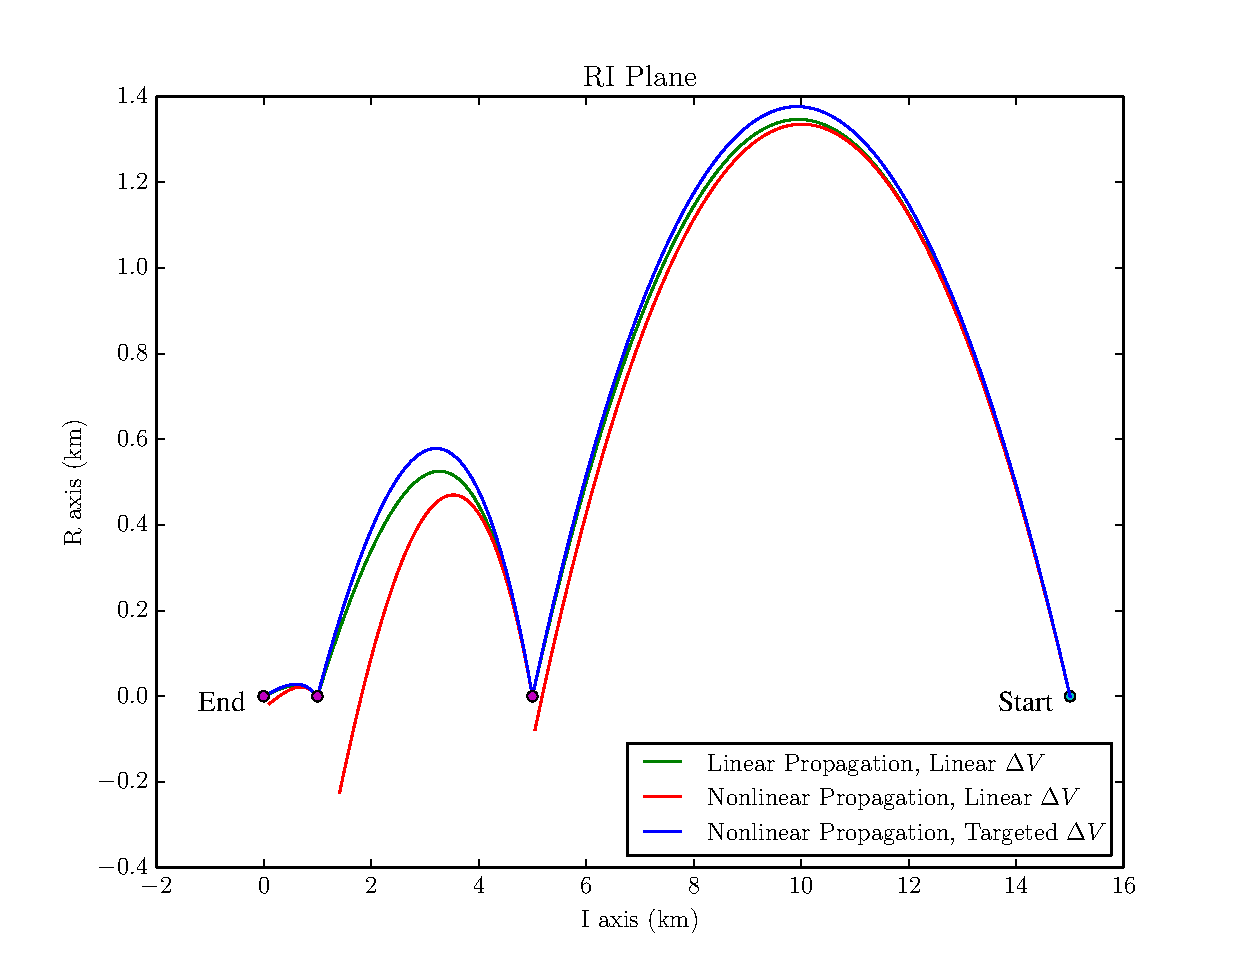
\includegraphics[width=0.9\textwidth]{RIC_1}
		\caption{Relative Motion of a Chaser Satellite with respect to a Target}
		\label{fig:RIC_1}
	\end{center}
\end{figure}

Not surprisingly, differences exist in the magnitude of the \(\Delta V\) between the linear computation and the nonlinear computation, as well as the angular difference between the two \(\Delta V\) vectors, and the resulting achieved position errors.  The robustness of the procedure, with respect to the convergence of the differential corrector using the initial guess from the linear model, also depends on properties of the rendezvous such as the time allowed and distance traveled between waypoints.

This technique is employed to evaluate the relative \(\Delta V\) cost of different rendezvous strategies.  Because of the differing local curvature of the target satellite's orbit as it progresses around its libration point, initiating a rendezvous at different starting points will affect the relative motion patterns of the rendezvous. In addition, approaching the target satellite from a different direction will also affect the \(\Delta V\) cost.  Results of various rendezvous approach strategies are presented.

\clearpage

\bibliographystyle{unsrt}
\bibliography{LPORendezvous}

\end{document}
